\subsection{Decomposition Strategies}
\label{subsec:decomposition-strategies}
To parallelize the Sobel filter, we implemented three decomposition methods to divide the computational domain among MPI ranks:
\begin{itemize}
    \item \textbf{Row-slab Decomposition:} The input image is divided horizontally into row-wise slabs, and each rank processes one row.
    \item \textbf{Column-slab Decomposition:} The input image is divided vertically into column-wise slabs, and each rank processes one column.
    \item \textbf{Tiled Decomposition:} The input image is divided into smaller rectangular tiles, where each rank processes one tile.
\end{itemize}

Figure~\ref{fig:decomposition-methods} illustrates these decomposition methods using a total of 16 ranks.

\begin{figure}[h]
    \centering
    \begin{subfigure}{0.3\textwidth}
        \centering
        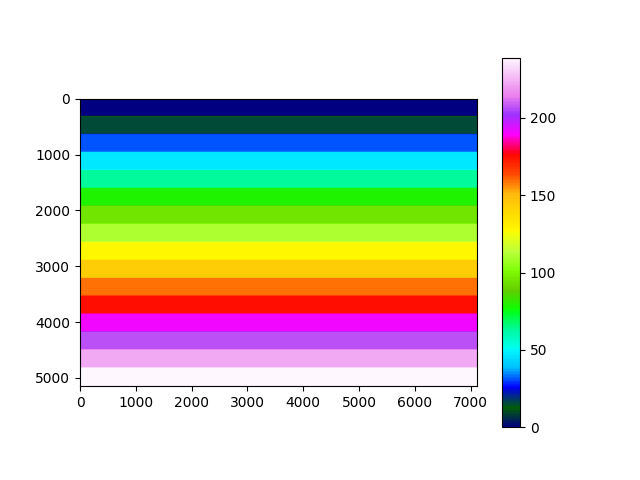
\includegraphics[width=\textwidth]{images/row_slab.png}
        \caption{Row-slab Decomposition}
        \label{fig:row-slab}
    \end{subfigure}
    \hfill
    \begin{subfigure}{0.3\textwidth}
        \centering
        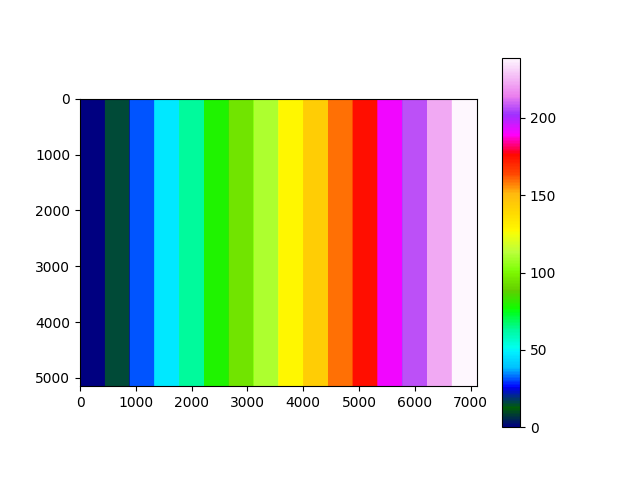
\includegraphics[width=\textwidth]{images/column_slab.png}
        \caption{Column-slab Decomposition}
        \label{fig:column-slab}
    \end{subfigure}
    \hfill
    \begin{subfigure}{0.3\textwidth}
        \centering
        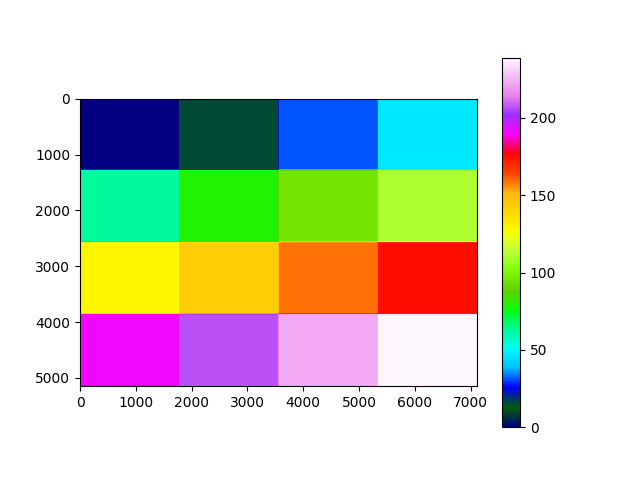
\includegraphics[width=\textwidth]{images/tiled.png}
        \caption{Tiled Decomposition}
        \label{fig:tiled}
    \end{subfigure}
    \caption{Graphical representation of the decomposition strategies (Row-slab, Column-slab, and Tiled) using a total of 16 ranks.}
    \label{fig:decomposition-methods}
\end{figure}